\documentclass[UTF8,twocolumn,a4paper]{ctexart}
\usepackage[margin=1.8cm]{geometry}
\usepackage{graphicx}
\usepackage{booktabs}
\usepackage{amsmath}
\usepackage{url}
\usepackage{hyperref}
\usepackage{caption}
\usepackage{float}

\title{\heiti 基于条件生成对抗网络的草图提示商品图像生成系统}
\author{黄正扬}
\date{\today}

\begin{document}
\maketitle

\begin{abstract}
本实验围绕图像到图像翻译任务，使用 Pix2Pix 条件生成对抗网络实现鞋类边缘草图到彩色商品图像的转换。模型采用 U-Net 作为生成器，采用 PatchGAN 作为判别器，并使用对抗损失和 L1 重建损失共同训练。实验数据来自 edges2shoes 数据集，训练时从原始数据中抽取 100 对图像，训练 5 个 epoch，并在 20 对图像上进行推理和评价。实验结果显示，模型的训练损失随 epoch 增加而下降，最终在评价集上得到 Mean L1 为 0.3447、PSNR 为 7.08、SSIM 为 0.3414。由于训练样本较少且仅使用 CPU 训练，生成图像的颜色和纹理细节仍比较粗糙，但整体流程能够完成从草图输入到商品图像输出的基本任务。
\end{abstract}

\noindent\textbf{关键词：}生成对抗网络；Pix2Pix；条件 GAN；图像到图像翻译；草图生成；深度学习

\section{引言}
生成对抗网络（Generative Adversarial Network, GAN）是生成模型中的一种重要方法。GAN 由生成器和判别器组成，生成器负责生成样本，判别器负责判断样本是真实数据还是生成数据。二者在训练过程中相互竞争，使生成器逐渐学会生成更接近真实数据分布的样本。

普通 GAN 通常从随机噪声生成图像，而本实验关注的是有条件的图像生成。对于草图到商品图像的任务，输入草图已经给出了鞋子的轮廓和主要结构，模型需要在此基础上补充颜色、明暗和局部纹理。Pix2Pix 是一种适合成对图像翻译任务的条件 GAN 方法，因此本实验选择 Pix2Pix 作为主要模型，在 edges2shoes 数据集上完成边缘草图到鞋类商品图像的转换。

\section{相关工作}
Goodfellow 等人提出的 GAN\cite{goodfellow2014gan} 通过生成器和判别器之间的最小最大博弈建立生成模型。该方法提出后，许多研究开始尝试将 GAN 用于图像生成和图像转换任务。条件 GAN 在 GAN 的基础上加入输入条件，使生成结果受到标签、图像或其他信息的控制。

Pix2Pix\cite{isola2017pix2pix} 将条件 GAN 用于成对图像到图像翻译，并在边缘图到真实图像、标签图到街景等任务上取得了较好的效果。CycleGAN\cite{zhu2017cyclegan} 则主要用于非成对图像数据，通过循环一致性约束学习两个域之间的映射。由于 edges2shoes 数据集本身提供了边缘图和鞋子照片的成对样本，本实验采用 Pix2Pix 会更直接，也更容易分析训练目标和实验结果。

\section{方法}
\subsection{任务定义}
设输入边缘草图为 $x$，目标商品图像为 $y$。实验希望训练一个生成器 $G$，使其输出 $G(x)$ 尽可能接近真实商品图像 $y$。判别器 $D$ 的输入是条件图像和目标图像的拼接，即 $(x,y)$ 或 $(x,G(x))$，输出用于判断目标图像是真实图像还是生成图像。

\subsection{生成器}
生成器采用 U-Net 结构。U-Net 由编码器和解码器组成，编码器逐层下采样以提取语义特征，解码器逐层上采样以恢复图像尺寸。U-Net 中的跳跃连接可以把浅层边缘信息传递到解码阶段，有助于保留鞋底、鞋面边界等结构信息。对于草图到图像任务，这种结构比普通编码器-解码器更适合保持输入轮廓。

\subsection{判别器}
判别器采用 PatchGAN 结构。PatchGAN 不直接给整张图像一个真假判断，而是对图像中的局部区域进行判断。这样做的好处是判别器能够更关注局部纹理和边缘连续性，同时参数量也相对较少。训练时，真实图像对记为正样本，生成图像对记为负样本。

\subsection{损失函数}
生成器的损失由两部分组成。第一部分是对抗损失，用于让生成图像尽可能骗过判别器；第二部分是 L1 重建损失，用于约束生成图像与真实目标图像在像素层面接近。实验中使用的目标函数为
\begin{equation}
\mathcal{L}_{G}=\mathcal{L}_{GAN}(G,D)+\lambda_{L1}\mathcal{L}_{1}(G),
\end{equation}
其中 $\lambda_{L1}=100$。L1 损失权重较大，可以让训练前期更稳定，也能使生成结果更贴近成对标注图像。

\section{数据集与实验设置}
实验使用 edges2shoes 数据集。该数据集中的每张图像由左右两部分拼接而成，一侧是鞋子的边缘图，另一侧是对应的鞋子照片。程序读取图像后会将其从中间切分，并按照 AtoB 的方向把边缘图作为输入，把真实鞋子照片作为目标图像。

本次实验在 CPU 环境下运行。训练集从原始数据集中抽取 100 对图像，评价时使用 20 对图像。主要训练参数如表 \ref{tab:setting} 所示。

\begin{table}[H]
\centering
\caption{主要实验参数}
\begin{tabular}{lc}
\toprule
参数 & 取值 \\
\midrule
输入尺寸 & $256\times256$ \\
训练样本数 & 100 \\
评价样本数 & 20 \\
训练轮数 & 5 \\
Batch size & 1 \\
学习率 & 0.0002 \\
$\lambda_{L1}$ & 100 \\
训练设备 & CPU \\
\bottomrule
\end{tabular}
\label{tab:setting}
\end{table}

评价指标使用 Mean L1、PSNR 和 SSIM。Mean L1 反映生成图像和目标图像之间的平均像素误差，PSNR 常用于评价重建质量，SSIM 用于衡量图像结构相似性。除了定量指标外，实验还保存了输入草图、目标图像和生成图像的三列对比图，用于观察生成效果。

\section{实现过程}
实验代码使用 PyTorch 编写。数据读取部分负责加载成对图像、切分左右半图、调整图像大小并归一化到 $[-1,1]$。模型部分包括 U-Net 生成器、PatchGAN 判别器和损失函数。训练过程中交替更新判别器和生成器，并在每个 epoch 后保存模型权重和损失记录。

推理阶段只使用训练好的生成器。程序读取测试图像中的边缘草图，输入生成器后得到彩色鞋子图像，再将输出反归一化并保存为普通图片。为了便于观察，程序同时保存 input、target 和 generated 三列对比图。评价阶段将 generated 文件夹中的图片与 target 文件夹中的图片按文件名匹配，然后计算 Mean L1、PSNR 和 SSIM。

\section{实验结果}
图 \ref{fig:loss} 展示了 5 个 epoch 的训练损失变化。从曲线和表 \ref{tab:loss} 可以看到，生成器总损失和 L1 损失在前两轮下降较明显，之后下降速度变慢。第 1 个 epoch 的 L1 损失为 36.9426，第 5 个 epoch 降到 18.3201，说明模型已经学到了一部分从边缘图到鞋子照片的对应关系。

\begin{figure}[H]
\centering
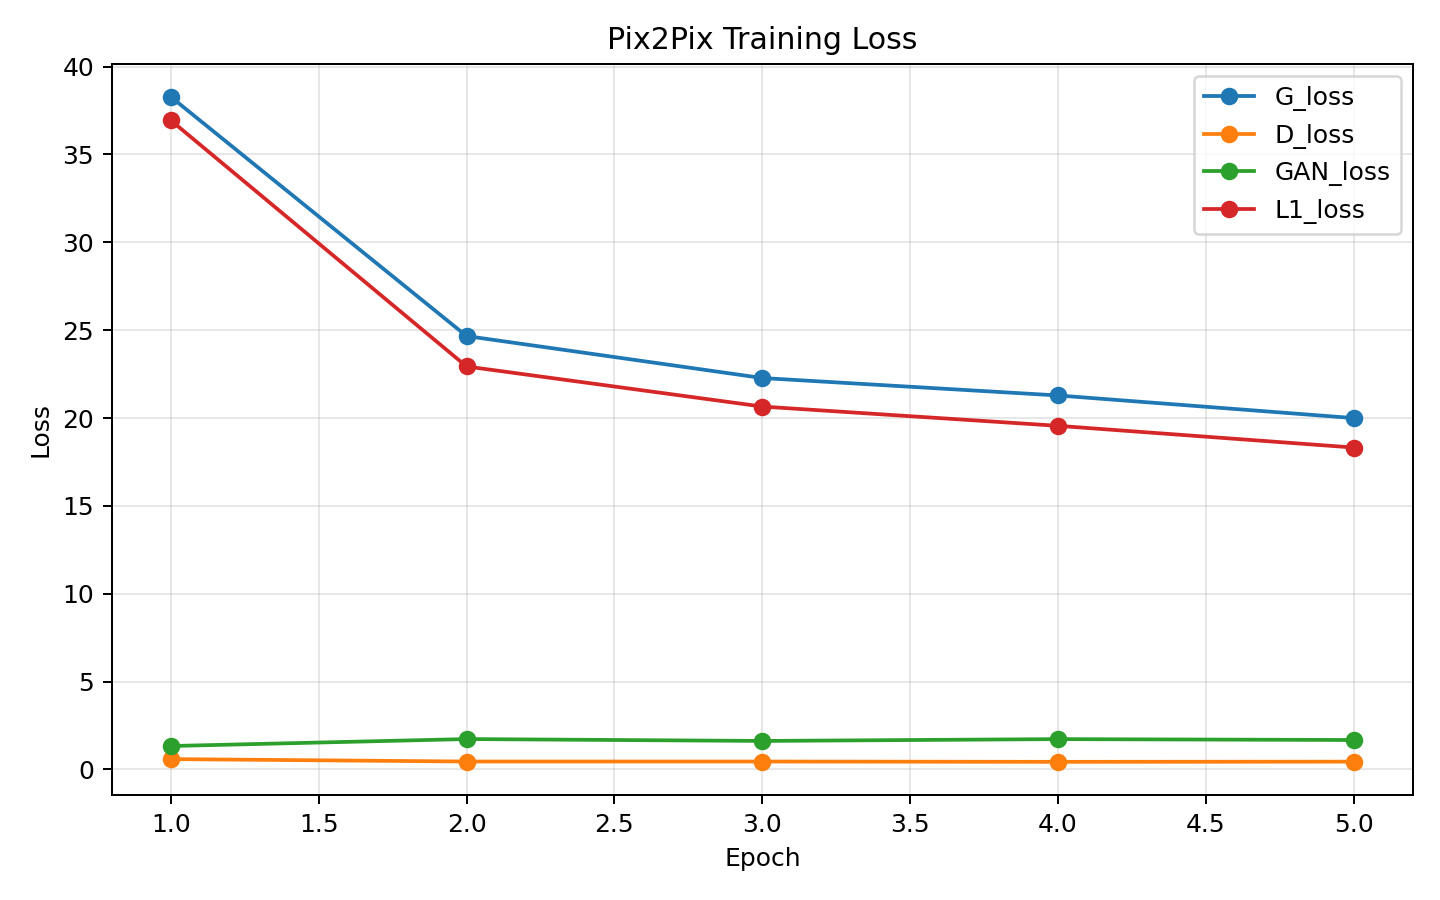
\includegraphics[width=\linewidth]{figures/loss_curve.png}
\caption{训练损失曲线}
\label{fig:loss}
\end{figure}

\begin{table}[H]
\centering
\caption{各 epoch 的平均损失}
\begin{tabular}{ccccc}
\toprule
Epoch & G loss & D loss & GAN loss & L1 loss \\
\midrule
1 & 38.2775 & 0.5904 & 1.3349 & 36.9426 \\
2 & 24.6648 & 0.4530 & 1.7312 & 22.9336 \\
3 & 22.2763 & 0.4526 & 1.6241 & 20.6521 \\
4 & 21.2839 & 0.4341 & 1.7277 & 19.5563 \\
5 & 19.9973 & 0.4454 & 1.6771 & 18.3201 \\
\bottomrule
\end{tabular}
\label{tab:loss}
\end{table}

图 \ref{fig:inference} 给出了部分推理结果。整体来看，生成图像能够大致跟随输入草图的鞋子轮廓，鞋底和鞋面的位置基本对应；但是图像的颜色不够稳定，纹理细节也比较模糊。这与训练样本较少、训练轮数较短有关。

\begin{figure}[H]
\centering
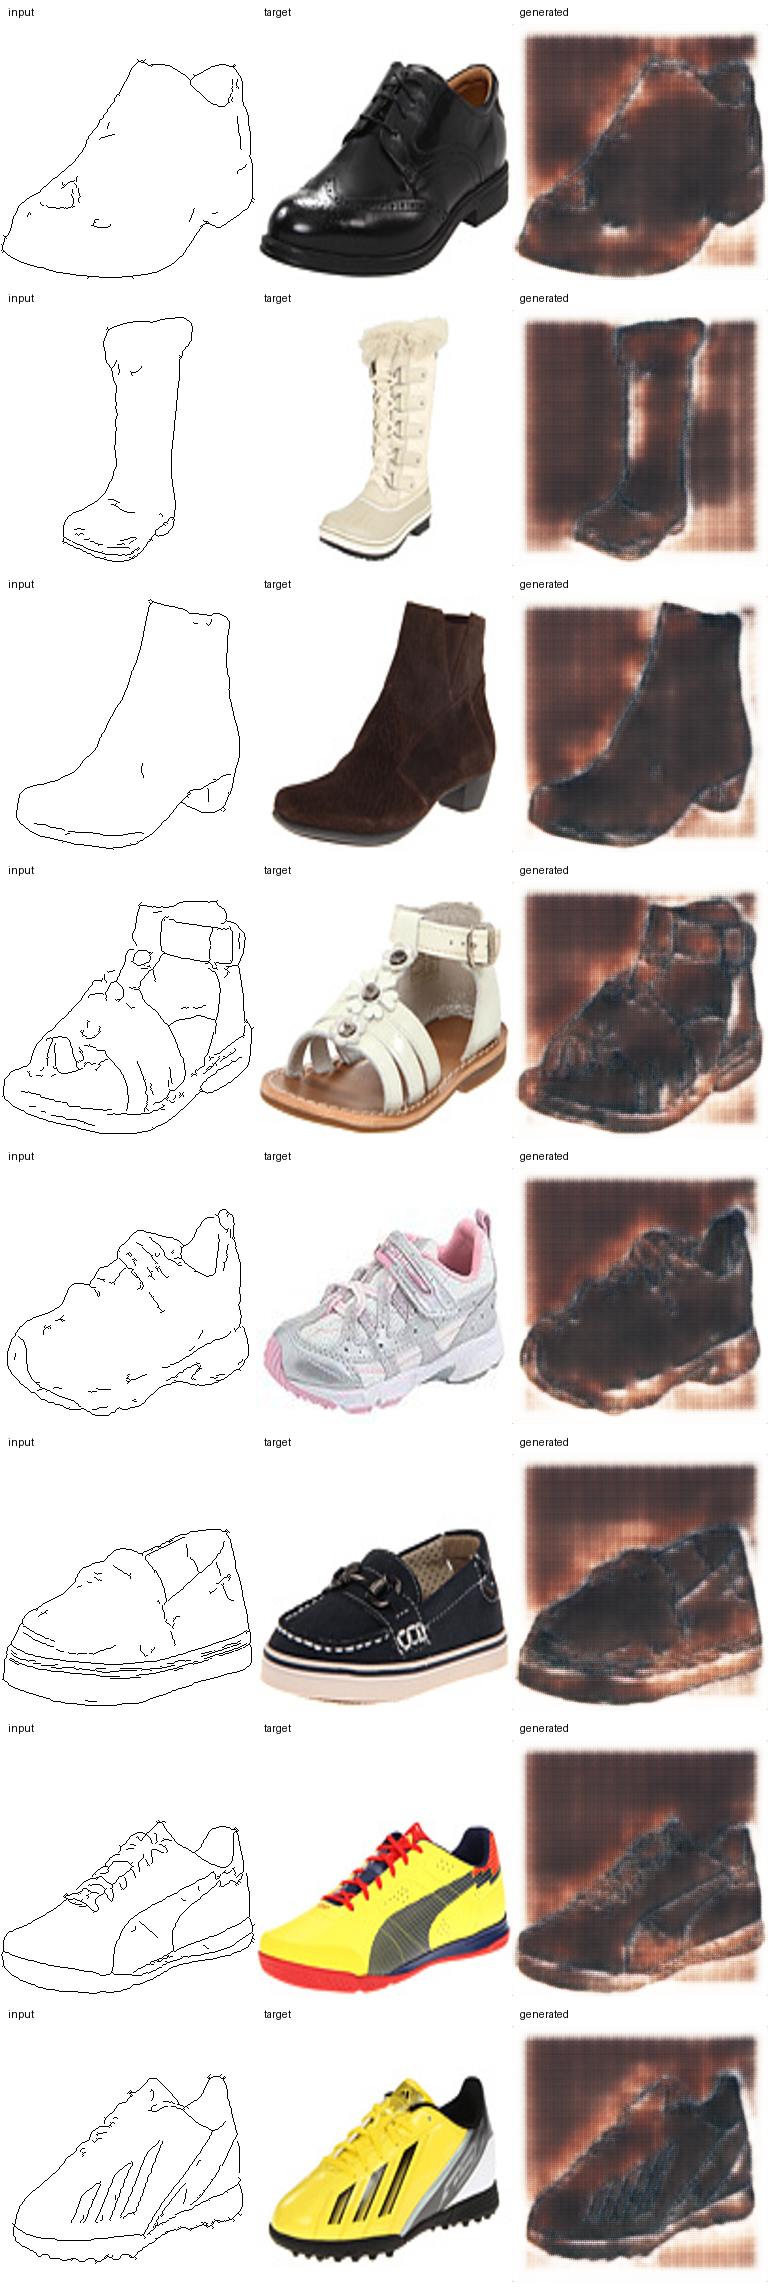
\includegraphics[width=\linewidth]{figures/inference_grid.png}
\caption{输入草图、目标图像和生成图像对比}
\label{fig:inference}
\end{figure}

表 \ref{tab:metrics} 给出了 20 对评价图像上的定量结果。Mean L1 为 0.3447，PSNR 为 7.08，SSIM 为 0.3414。从数值看，模型还没有达到较高的重建质量，但已经能够完成基本的图像翻译过程。

\begin{table}[H]
\centering
\caption{评价指标结果}
\begin{tabular}{lccc}
\toprule
样本对数 & Mean L1 $\downarrow$ & PSNR $\uparrow$ & SSIM $\uparrow$ \\
\midrule
20 & 0.3447 & 7.08 & 0.3414 \\
\bottomrule
\end{tabular}
\label{tab:metrics}
\end{table}

\section{结果分析}
从训练损失可以看出，L1 损失在 5 个 epoch 内有比较明显的下降，说明生成器逐渐学会了根据边缘图恢复目标图像的大致结构。第 2 个 epoch 以后损失下降变慢，说明在 100 张训练样本的设置下，模型很快学到了较容易的轮廓对应关系，但更细的颜色和纹理仍然难以学习。

从可视化结果看，生成图像的主要问题是细节不清晰，部分区域颜色偏灰或过于平滑。这与 Pix2Pix 中 L1 损失的特点有关：L1 损失会鼓励像素平均意义上的接近，但在纹理较复杂时容易得到平滑结果。对抗损失可以在一定程度上改善局部真实感，但在小样本训练下判别器本身也不够稳定。

本次实验使用 CPU 训练，因此没有继续扩大训练轮数。若在 GPU 环境下训练，可以使用更多 edges2shoes 样本，并把 epoch 增加到几十轮。预计在数据量和训练时间增加后，模型对颜色和材质的学习会更充分，生成图像的细节也会更清楚。

\section{交互界面}
为了便于展示，实验还编写了一个简单的 Web 演示界面。界面允许用户上传一张边缘草图，点击生成按钮后调用训练好的生成器输出鞋类商品图像。该界面主要用于展示模型的推理过程，实际生成质量仍取决于训练好的模型权重。

\begin{figure}[H]
\centering
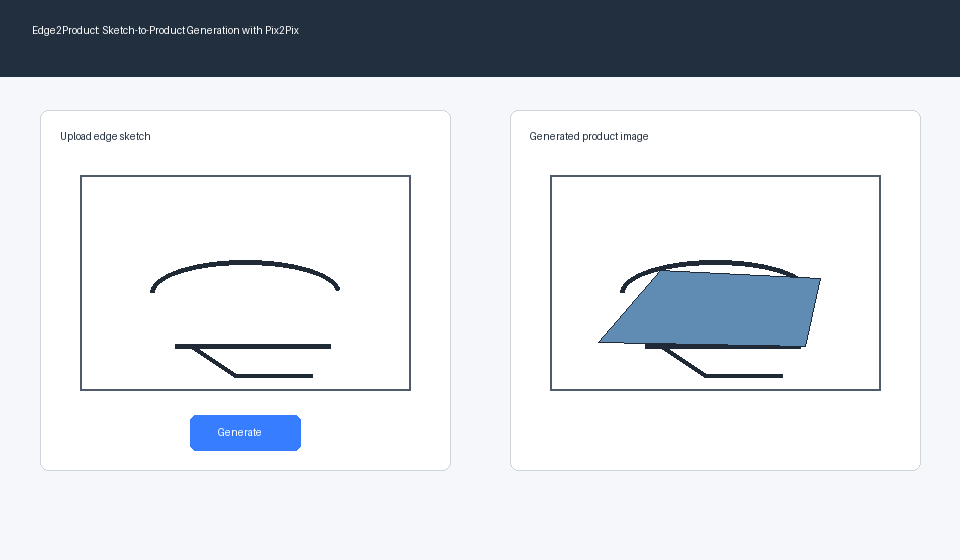
\includegraphics[width=\linewidth]{figures/ui_screenshot_placeholder.png}
\caption{交互界面示意图}
\label{fig:ui}
\end{figure}

\section{不足与改进}
本实验的主要不足是训练规模较小。100 对样本不足以覆盖鞋子外观的多样性，5 个 epoch 也不足以让 GAN 训练充分收敛。此外，Pix2Pix 依赖成对数据，如果应用到没有配对图像的数据集，需要考虑 CycleGAN 等非成对图像翻译方法。

后续可以从三个方面改进。第一，使用 GPU 训练更多样本和更多 epoch；第二，在损失函数中加入感知损失或特征匹配损失，以改善纹理细节；第三，和 CycleGAN、CUT 等方法做对比实验，分析不同图像翻译方法在草图到商品图像任务上的差异。

\section{总结}
本实验实现了基于 Pix2Pix 的鞋类边缘草图到商品图像生成。通过训练 U-Net 生成器和 PatchGAN 判别器，模型能够根据输入草图生成大致符合轮廓的鞋子图像。实验结果表明，在 100 张训练样本和 5 个 epoch 的设置下，损失有下降趋势，但生成图像仍存在颜色不稳定和纹理模糊的问题。通过本次实验，我对条件 GAN、Pix2Pix 模型结构、成对图像数据处理以及生成模型评价指标有了更直观的理解。

\bibliographystyle{unsrt}
\bibliography{references}

\end{document}
